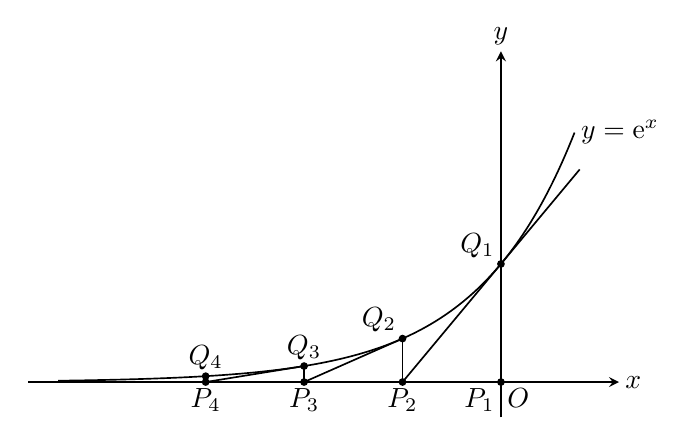
\begin{tikzpicture}[x=1.25cm,y=1.5cm,line width=.6pt,>=stealth]
\draw[->] (-4.8,0)--(1.2,0) node[right,inner sep=0pt,xshift=2pt] {$x$};
\draw[->] (0,-0.3)--(0,2.8) node[above,inner sep=0pt,yshift=2pt] {$y$};
\draw[domain=-4.5:0.75,samples=160] plot (\x,{exp(\x)});
\draw (0,0)--(0,1);
\draw (-1,0)--(-1,0.3679);
\draw (-2,0)--(-2,0.1353);
\draw (-3,0)--(-3,0.0498);
\draw (0,1)--(-1,0);
\draw (-1,0.3679)--(-2,0);
\draw (-2,0.1353)--(-3,0);
\draw (0,1)--(0.8,1.8);
\fill (0,0) circle[radius=1.4pt];
\fill (-1,0) circle[radius=1.4pt];
\fill (-2,0) circle[radius=1.4pt];
\fill (-3,0) circle[radius=1.4pt];
\fill (0,1) circle[radius=1.4pt];
\fill (-1,0.3679) circle[radius=1.4pt];
\fill (-2,0.1353) circle[radius=1.4pt];
\fill (-3,0.0498) circle[radius=1.4pt];
\node[below left,inner sep=0pt,xshift=-2pt,yshift=-2pt] at (0,0) {$P_{1}$};
\node[below,inner sep=0pt,yshift=-2pt] at (-1,0) {$P_{2}$};
\node[below,inner sep=0pt,yshift=-2pt] at (-2,0) {$P_{3}$};
\node[below,inner sep=0pt,yshift=-2pt] at (-3,0) {$P_{4}$};
\node[above left,inner sep=0pt,xshift=-2pt,yshift=2pt] at (0,1) {$Q_{1}$};
\node[above left,inner sep=0pt,xshift=-2pt,yshift=2pt] at (-1,0.3679) {$Q_{2}$};
\node[above,inner sep=0pt,yshift=2pt] at (-2,0.1353) {$Q_{3}$};
\node[above,inner sep=0pt,yshift=2pt] at (-3,0.0498) {$Q_{4}$};
\node[below right,inner sep=0pt,xshift=2pt,yshift=-2pt] at (0,0) {$O$};
\node[right,inner sep=0pt,xshift=2pt] at (0.75,2.117) {$y=\mathrm{e}^{x}$};
\end{tikzpicture}
